\documentclass[conference,compsoc]{appendix/report}
\usepackage{graphicx, multirow} 
\ifCLASSOPTIONcompsoc
  % IEEE Computer Society needs nocompress option
  \usepackage[nocompress]{cite}
\else
  \usepackage{cite}
\fi

\ifCLASSINFOpdf
\else
\fi
\hyphenation{op-tical net-works semi-conduc-tor}

\begin{document}

\title{Report of ASC Student Supercomputer Challenge 2017 Preliminary Contest}

\author{\IEEEauthorblockN{Zhibin Xie, Zhen'ning Wang, Jiafang Xue, Guohua Tian}
\IEEEauthorblockA{School of Information Engineering,\\ NanChang University}

\and

\IEEEauthorblockN{Xianling Dong}
\IEEEauthorblockA{School of Science,\\NanChang University}

}

\maketitle

% \begin{abstract}
% -- NSBSS.
% \end{abstract}
% \IEEEpeerreviewmaketitle

\section{Super Computing At Nanchang University}

Nanchang University (NCU), recognized as one of the key university in Project 211 in the mid-western region of China, has shifted the focus on the education of cutting-edge technology and frontier research. In college of information science and technology, we provide undergraduate programs that allow student to know, touch, and
learn about high performance computing and Big Data analysis, with the focus on the computation ablity.
We have recently investigate multiple local and nation-wide sponsored projects on supporting advancing super computing in both research and education. In research, our university builds small scale computing clusters (i.e., over 20 nodes) to simulate near-space simulation and emulation in both 2D and 3D layout.
The scale of the computing platform has been scaled up last year after our college of information and technology further investigate over 3million Yuan for cluster upgrade using the Inspur scientific computing
solutions. To further exploit the capacity of super computing, we also offload large amounts of computation jobs onto the TianHe II platform. In this way, we build a distributed scientific computing hierarchy as local algorithm test/data verification, and remote hardcore high performance computing.

In the aspect of education, we also provide free charge platform to support students who are interested in super computing and data engineering. We have investigated 1.7 million to build a micro datacenter with 30 computation nodes, 8 storage nodes with network-attached storage (NAS), and rest manage nodes. The purposes of building such platform are three folds: (1) Provide a sandbox of raw Linux system/HPC hardware/machine learning frameworks for student to play with; (2) Build a syllabus around high performance computing in order to train engineers, and possibly researchers in this field; (3) Support education-related research on high performance computing. In three months, we have over 50 undergraduate and 15 graduate students working on this platform to study, manage, do research, and work on their thesis. This is a relatively new trend on the revolutionize the out-of-date courses, and now combined into the most recent technique and system designs.

\subsection{On-going Grant-support Projects}

The super computing platform in NCU is currently supporting multiple on-going research projects. Research sponsored by National Science Foundation China (NSFC) and Jiangxi Provincial department of science and technology can be separated into three major categories. The first category is the scientific computing research on space science and technology, with a focus on near-space simulation, and Terahertz radiation application. The second group of on-going research are image processing and computer vision projects on Big data, such as medical images and records. Our professors use deep learning methods to explore and discover symptoms from CT/MRI images to help symptom diagnose and remote surgery. The last group focuses on the computation capacity. The research is mainly focus on how to build an efficient yet effective computing architecture to support the aforementioned two groups of research by draining every possible drop of computation frequency and I/O bandwidth, such that the latency is minimized while the correctness and stability of the system are preserved.


\section{Introduction of NSBSS}
We are a group of youths loving computer science who have a
huge dream, and working hard for reaching higher. We gathered
together due to strong interest in supercomputer.\\
It is very happy to us that we have get together to take challenge of ASC17, and it is a good chance to get skills and knowledge about supercomputer.\\



% ------HPL Test------

\section{HPL Test}
\subsubsection{System environment}
\begin{tabular}{|c|c|}
\hline
Name & Configuration \\
\hline
\multirow{3}{*}{Inspur NF6248 } & CPU:Intel Xeon Phi 7210, 1.3Ghz, 64 cores \\ 
& Memory: 16G x4, DDR4, 2133Mhz \\
& Hard disk: 120G SSD x 1\\
\hline
\end{tabular}
\newline
\newline

\noindent \begin{tabular}{|c|c|c|}
\hline
Classification & Description & Version \\
\hline
OS & Linux & CentOS7 \\
\hline
Compiler & Intel Composer & 2017.1.043 \\
\hline
MKL & Intel MKL & 2017.1.043 \\
\hline
MPI & Intel MPI & 2017 UP1 \\
\hline
PBS & Torque &\\
\hline
\end{tabular}
\newline
\newline
\newline
% Details of HPL Test, such as MAX score, config and so on...\\
% I wish you the best of success.
\subsubsection{HPL install}

In this test and optimize, we chose Intel® Optimized LINPACK. \\

\subsubsection{Test Step}

\subsubsection{PxQ}

Because Intel® Optimized LINPACK use all CPU core in multi-thread
by default, so we set P x Q to 1 x 1. \\

\subsubsection{BLAS}
There are many blas, such as openblas, mkl, gogoblas and atlas.
Because we are using intel xeon phi, MKL will be the best choice \\

\subsubsection{N}
Experience tells us, N can be calculated by 
\[ N^2 * 8 = MEM * 80\% \]

so N should have been  82900, but in our test, when N is set to \\
35000, GFlops reach to 1.7GFlops, which is much higher when N is 829000 \\

\noindent \begin{tabular}{|c|c|c|c|c|c|c|}
\hline
N &  33000 & 34000 & 35000 & 36000 & 37000  \\
\hline
GFlops  &1702 &1701.48 &1714.1 &1708.11 &1501.21 \\
\hline
Time (S) &14.08 &15.4 &16.68 &18.21 &22.5 \\
\hline 
\end{tabular}
\newline
\newline
\par
\subsubsection{NB}
\noindent \begin{tabular}{|c|c|c|c|}
\hline
NB & 232 & 256 & 296 \\
\hline
GFlops & 1709.86 & 1714.1 & 1702.39 \\
\hline
\end{tabular}

\subsection{Best Score}
Finally, we reached at 1.7Gflops.  \\
\includegraphics[scale=0.35]{appendix/hpl.png}
\subsection{Problems}
Problem one, when N is set to theoretical size, the GFlops goes down straight. 

When we used multi-node, the performance become lower than we run the test on single-node, its confusing to us very much.

% ------MASNUM_WAVE------

\section{MASNUM\_WAVE}
% no \IEEEPARstart
\subsection{Ask question}
Question one,we use the queue of our team running exp1 and exp2. Then we get two files and verify them with standard results, but the makefile of verifica can't run in the folder of masnum\_wave. we compare pac\_ncep\_wav\_20090228.nc to pac\_ncep\_wav\_20090228\_stardard.nc and compare global\_ncep\_wav\_20090630.nc to globalncep\_wav\_20090630\_stardard.nc. Them compare success. But when we start to compare them, we begin to make the makefile, then run executable file compare\_exp1 getting a result "-bash: ./compare\_exp1: connot execute binary file". 
Question two, we use qsub to submit job and need to find the best flags for it.
Question three, when we use mpi + OpenACC* to optimize source code, and we test source code finding that the function of mpi\_reduce() and mpi\_bcast() which locate 251 line and 252 line in the file of source/ympi\_mod/ympi\_mod.f90 use the most time, mainly to input data to cache. However, when we use OpenAcc* to optimize the /source/ympi\_mod/wammpi\_mod.f90, we get errors. You can see following pictures in appendix A.

\subsection{Analyze problems}
Firstly,  Ocean wave model, we need to solve the optimization problem is how to ensure the accuracy of the case, the forecast to spend the shortest time. The main problems are code optimization, mathematical optimization, compiler selection, and the use of qsub to submit tasks, the need for parameter selection and other issues, code optimization is to Fortran language loop optimization, function call optimization, mathematical optimization is mainly marine wave prediction Formula optimization. The choice of the compiler is mainly to optimize the parallelization.

\subsection{Solve problems}
quetion one, We find the reason , because the compiler make us get fault. After we use gfortran compiler to make makefile and run success. And question two, we are step by step to test the best flags.  Our qsub submit command which is "bsub -n 64 -np 4 -p -q q\_sw\_asc\_2 -share\_size 7500 -host\_stack 1024 -b -m 1 -o out.qrunout -cgsp 64 ./masnum.wam.mpi", We use Mpi + OpenACC* to optimize our source code. You can see following pictures in appendix A.
\subsection{Get conclusion}
Now we optimize exp1 get result which is five hours, about five minutes to forecast a day, finishing job spend five hours. But we can't slove error of using OpenACC* optimization. can see last one picture following in appendix A.

% ------PaddlePaddle------

\section{Deep learning contest}
In-depth learning is a learning algorithm that simulates the cognitive pattern of the human brain, and the current Baidu Research Institute uses the strategic direction of data mining and artificial intelligence as an important development strategy of the 21st century.

PaddlePaddle is originated in Baidu's open source depth learning platform.And it's easy to use.

\subsection{Analysis of the problem}
Data are sampled from mobile phone APP.Using the dataset which are aggregated about 50 days from 00:00 a.m. on March 1st to 08:00 on April 20th for training. Your task is to predict each link's speed for every 5 minutes from 08:00 to 10:00 on April 20th.

The model outputs are evaluated by the Root Mean Squared Error (RMSE) of
predictions.

$$RMSE = \sqrt{\frac{ \sum_{i=1}^{n} \left ({X}_{actual, i}\footnotemark [1] - {X}_{model, i}\footnotemark [2] \right )^{2}}{n} }$$

\footnotemark [1]{ ${X}_{actual, i}$ is actual value of moment i, }

\footnotemark [2]{${X}_{model, i}$,i is your prediction moment of i}
\\
\\
By simply observing the node graphs, we map the traffic nodes, for example, simple crossroads

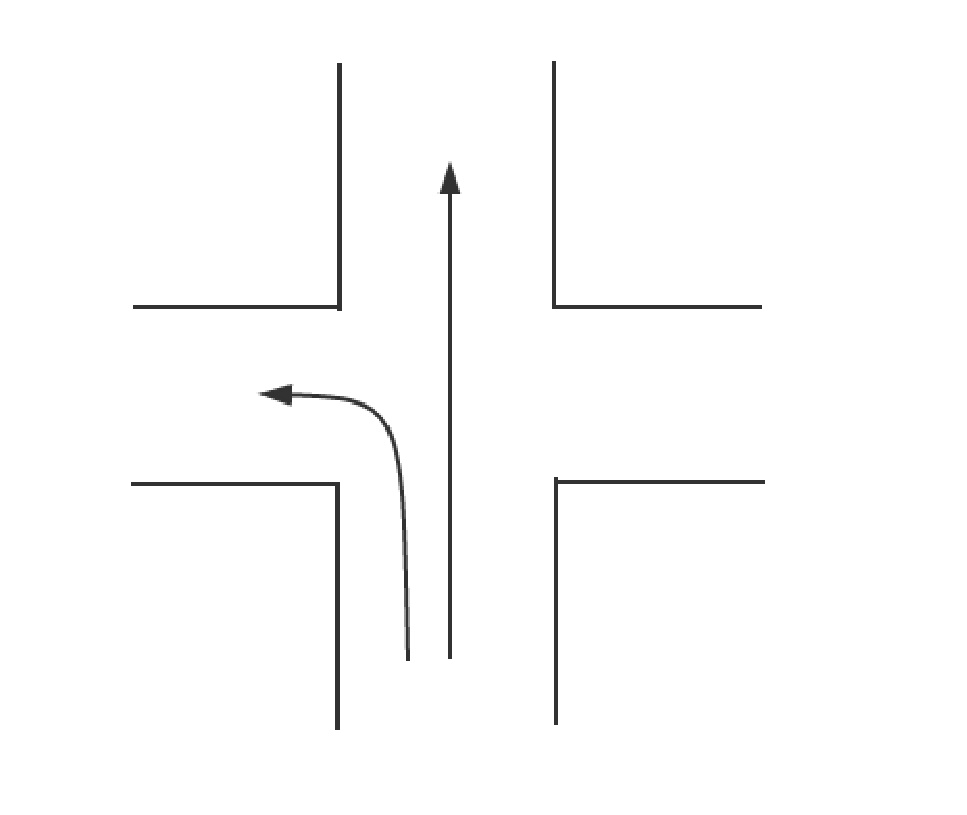
\includegraphics[width=3.00in,height=2.00in]{appendix/crossroads.eps}

Corresponding to the four traffic states.

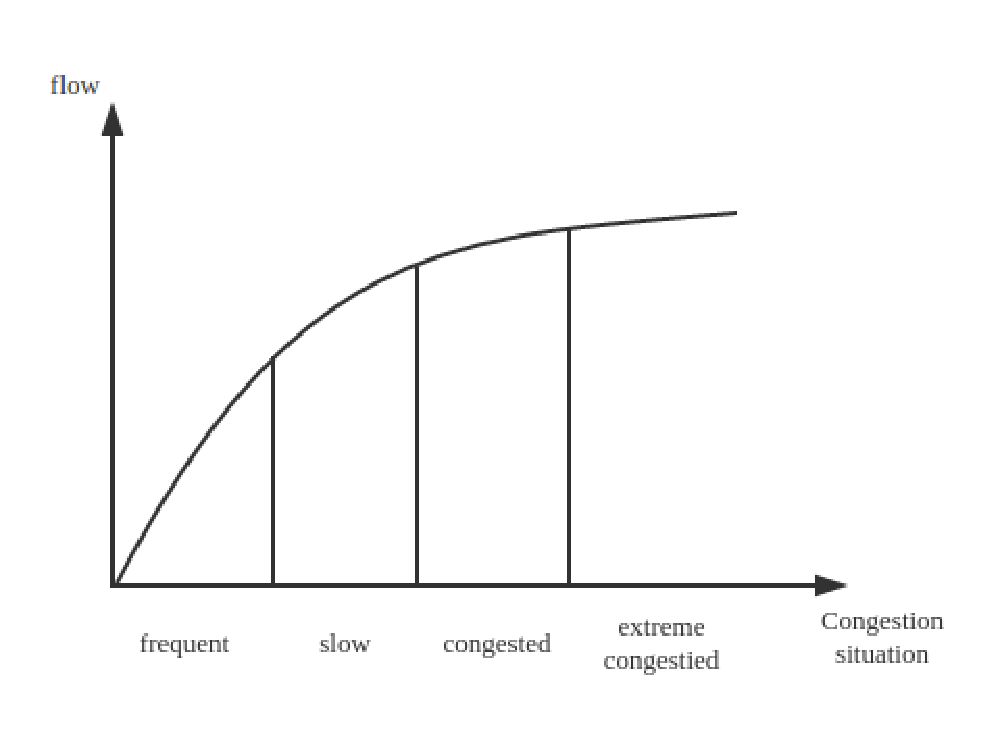
\includegraphics[width=3.00in,height=2.00in]{appendix/states.eps}

The result of clustering is the four eigenvectors (1, 2, 3, 4) corresponding to the state defined by the topic. The four eigenvectors represent frequently, slow, congested and extreme congested.

\subsection{Questions}
After we downloaded the data, we found that the amount of data is large, some of the data there is a large interference, so the data processing is very important.We also have little understanding of the depth of learning. so it is difficult to find theoretical support.
And the results of the prediction, and the calculation is unclear.


\subsection{Preliminary solution}
\subsubsection{Data processing}
Through the analysis of the title and data, we selected the daily time from 00:00-02:00, 04:00-06:00, 08:00-10:00, 12:00-14:00, 16:00-18:00 and 20:00-22:00 six time periods as the representative.In order to reduce the error, we take the average of the time to process the data.

For examples, March 7th and April 6th. These images have similar places

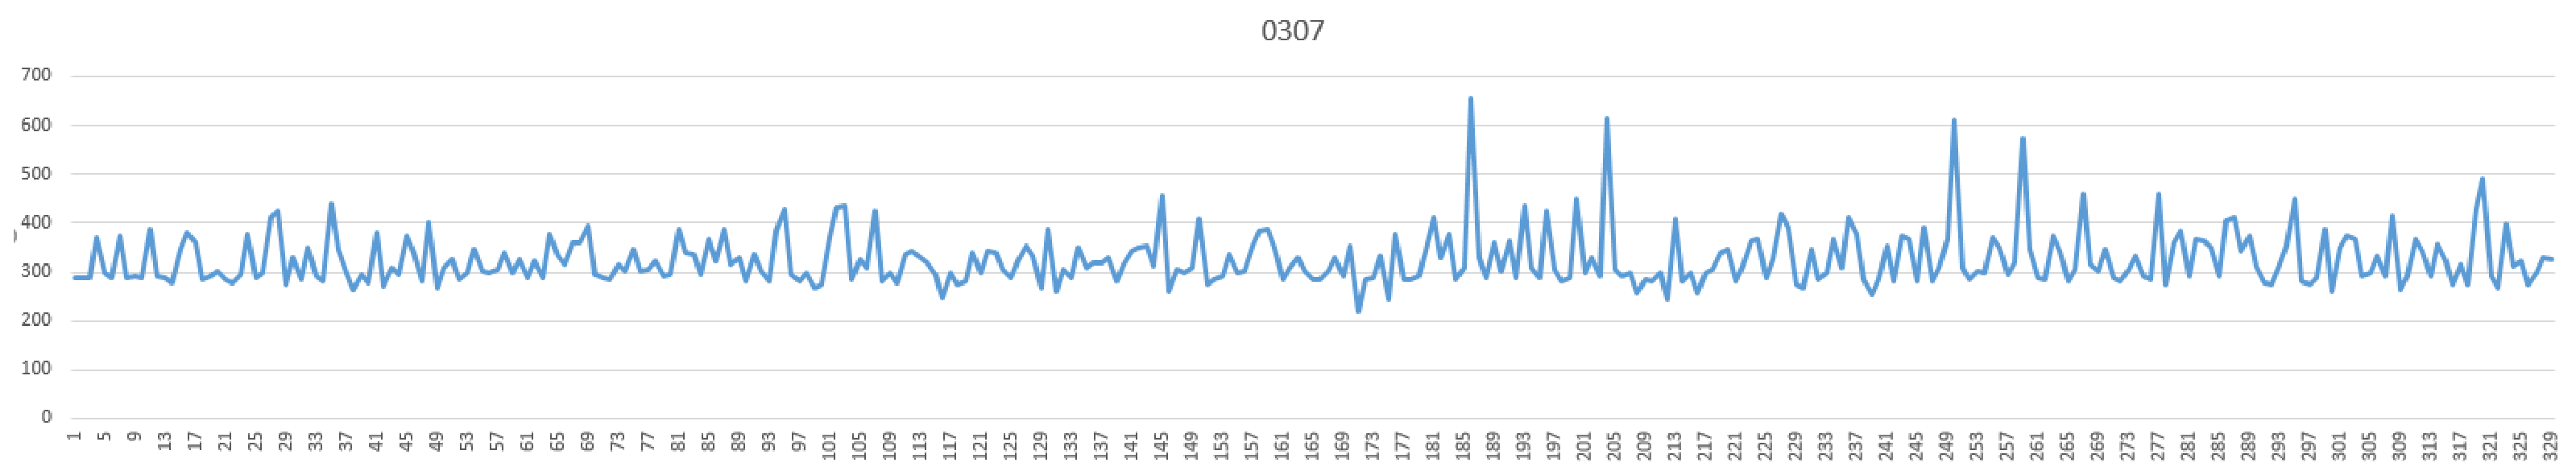
\includegraphics[width=3.00in,height=2.00in]{appendix/0307.eps}

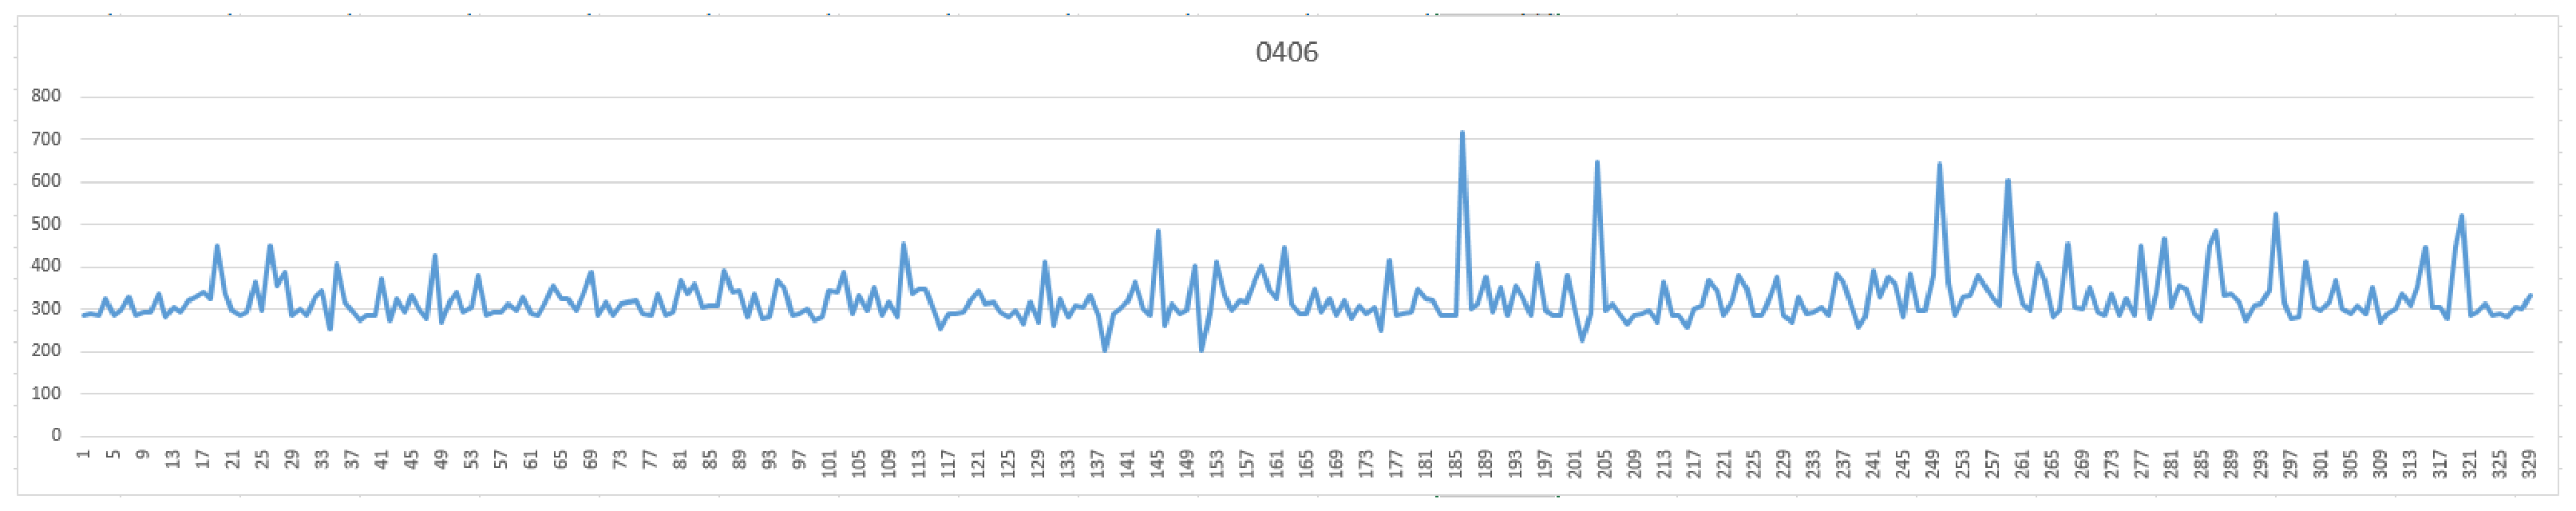
\includegraphics[width=3.00in,height=2.00in]{appendix/0406.eps}
\subsubsection{Algorithm selection}
Algorithm we used RMSProp, RMSProp is a very efficient algorithm, RMSProp slightly improved AdaGrad, making the algorithm no longer as radical as AdaGrad it is moving average of squared gradients.
\\
\\
The equations of this method as follows:

$$ \nu\left (w, t \right ) = \rho \nu\left ( w, t - 1 \right ) + \left ( 1 - \rho \right )\left ( 
\nabla{Q}_{i}(w) \right )$$

$$ w  = w - \frac{\eta }{\sqrt{\nu (w, t) + \varepsilon }} \left ( \nabla{Q}_{i}(w) \right )$$

\subsubsection{Result analysis}
We perform the error analysis by plotting the original data, and comparing the resulting data
\\
\\
Relative error:
$$ rerr = \frac{{X}_{actual, i} - {X}_{model, i}}{{X}_{actual, i}} $$
\\
\\
Absolute relative error:
$$ mrerr = \frac{1}{N} \sum_{1}^{N}\left ( \frac{{X}_{actual, i} - {X}_{model, i}}{{X}_{actual, i}} \right ) $$


\subsection{Algorithm improvement}
Adam is a recently proposed algorithm that is similar to the RMSprop comparison with the momentum. The procedure is similar to:


$$m(w,t) = {\beta}_{1} m(w, t - 1) + (1 - {\beta}_{1})\nabla{Q}_{i}(w)$$
$$v(w,t) = {\beta}_{2} v(w, t - 1) + (1 - {\beta}_{2})(\nabla{Q}_{i}(w))^{2}$$
$$w  = w - \frac{\eta }{\sqrt{\nu (w, t) + \varepsilon }}$$

The only difference between this method and RMSProp is the "smooth" process, which uses m to do the smooth operation instead of using the original gradient vector dx.And we set eps=1e-6, bata1=0.9, beta2=0.999.


\subsection{Parameter configuration}
Choose a suitable learning rate is very difficult, in the beginning, we set the way through the schedule learning learning method, that is pre-designed a certain series of iterations to increase or increase learning rate.As the learning rate increases, we find that the relative error begins to increase.Finally we set the learning rate to 1e-6.

\subsection{Cluster training}
As little understanding of the GPU, we only refer to the PaddlePaddle document cluster training related to the introduction and methods.Due to the lack of knowledge at the hardware level, we encountered many problems when we built the cluster.

\subsection{Result}
%表格
\begin{table}[h]  %table 里面也可以嵌套tabular,只有tabular是不能加标题的
\centering  %表格居中
\caption{模拟实验}  %表格标题
 \begin{tabular}{rrrr}  %右对齐
     \hline
     \hline
       & $learngin\_rate$ & ${rerr}_{i}$ & ${mrerr}_{i}$ \\ [0.5ex]  %增加行宽
       \hline
       1 & 1e-1 &   &   \\
       2 & 1e-2 &   &   \\
       3 & 1e-3 &   &   \\
       4 & 1e-4 &   &   \\
       5 & 1e-5 &   &   \\
       6 & 1e-6 &   &   \\
       7 & 1e-7 &   &   \\
       8 & 1e-8 &   &   \\
       \hline
       \multicolumn{2}{c}{Total Sqerr} &   &   \\  %横向合并两个单元格
       \hline
       \hline
   \end{tabular}
\end{table}
%结束

\subsection{Summary}
Due to the lack of relevant knowledge, our theoretical support is insufficient, the accuracy of the results can not be estimated, the actual accuracy is not very accurate.

% -----Conclusion-----

\section{Conclusion}
No conclusion yet...

% ----Appendix-----

\section{Appendix}

\subsection{A.}
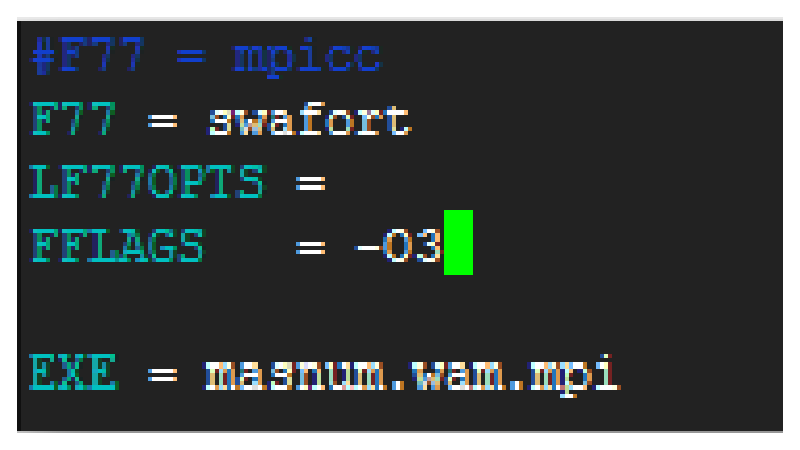
\includegraphics[width=3.50in,height=3.00in]{appendix/q28.eps}
\includegraphics[width=3.50in,height=3.00in]{appendix/q22.eps}
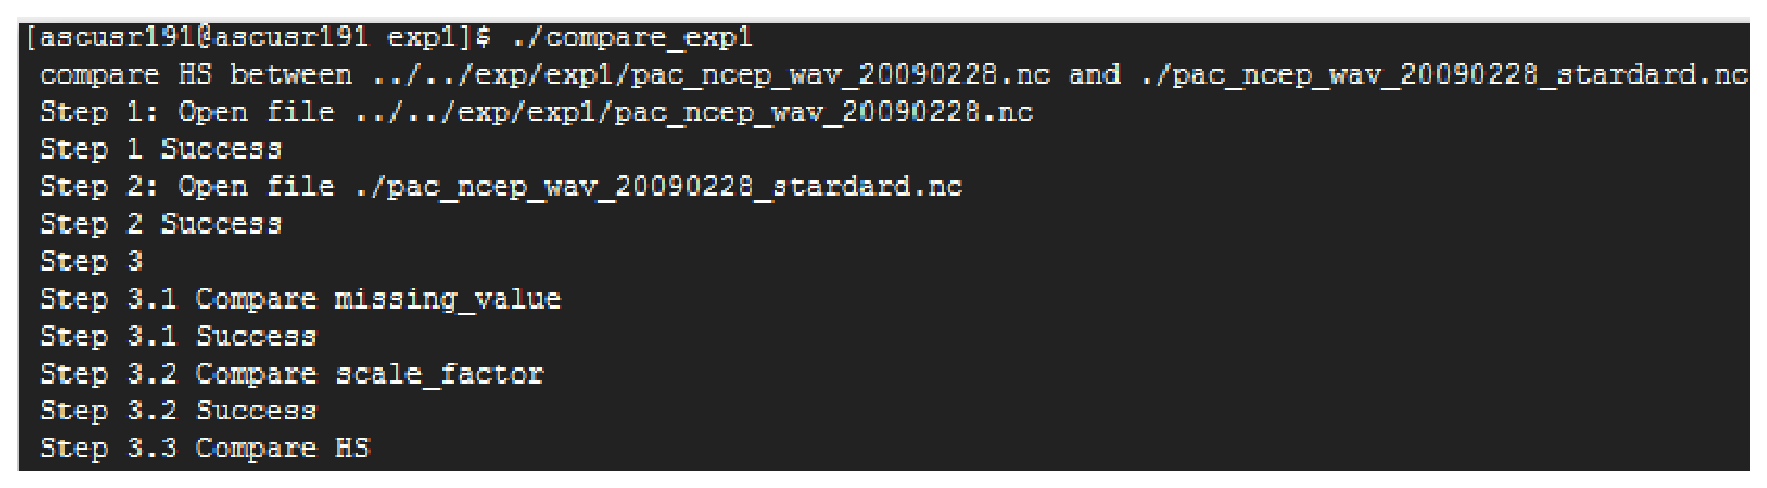
\includegraphics[width=3.50in,height=3.00in]{appendix/q25.eps}
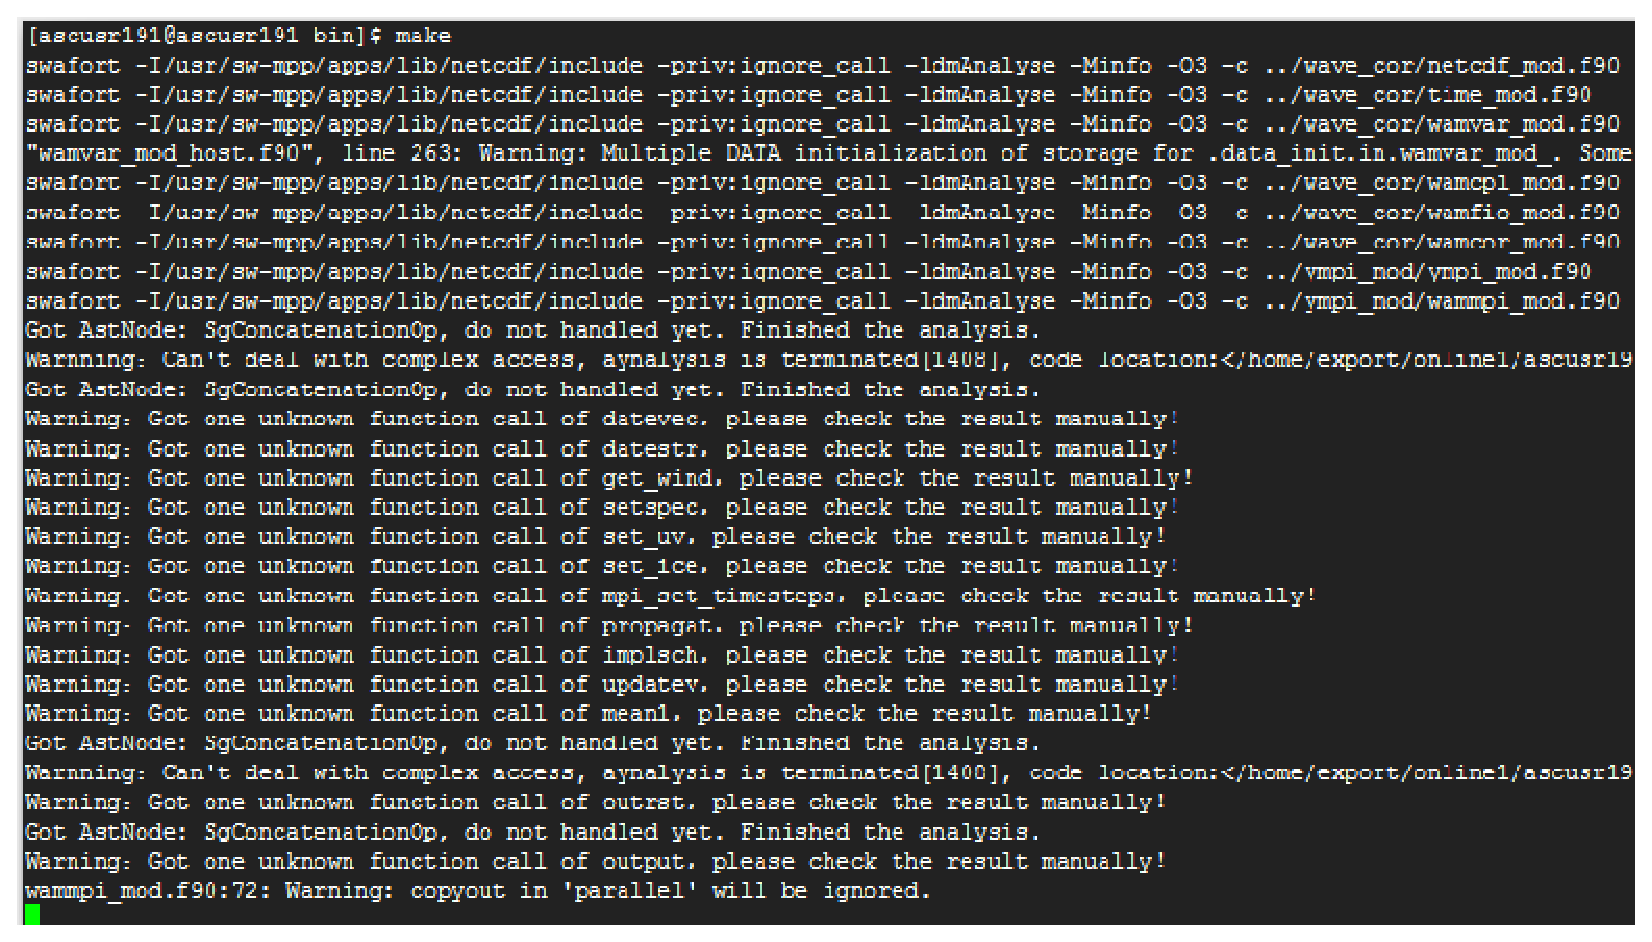
\includegraphics[width=3.50in,height=3.00in]{appendix/q26.eps}
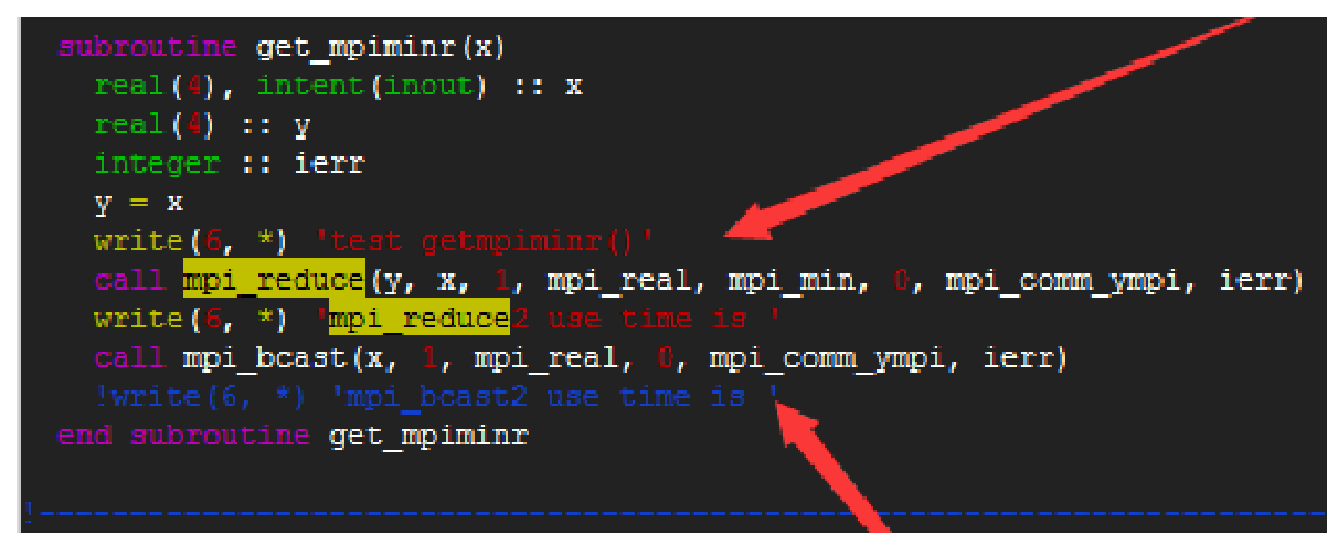
\includegraphics[width=3.50in,height=3.00in]{appendix/q24.eps}


% ---- References----

\begin{thebibliography}{1}

\bibitem{IEEEhowto:kopka}
H.~Kopka and P.~W. Daly, \emph{A Guide to \LaTeX}, 3rd~ed.\hskip 1em plus
  0.5em minus 0.4em\relax Harlow, England: Addison-Wesley, 1999.\\

\bibitem{IEEEhowto:kopka}
XunqiangYin. A highly effective global surface wave numerical simulation with ultra-high resolution

\bibitem{IEEEhowto:kopka}
Yongzeng Yang and Xunqiang Yin. User Guide for MASNUM-WAM 2.2(2010-07-10)

\bibitem{IEEEhowto:kopka}
J. Kraus. NVIDIA, Multi GPU Programming with MPI and OpenACC(2016-10-26)

\bibitem{IEEEhowto:kopka}
National Supercomputing Center in Wuxi. Sunway TaihuLight Quick Start Guide

\bibitem{IEEEhowto:kopka}
National Supercomputing Center in Wuxi. Sunway TaihuLight OpenACC* Quick User Handset

\bibitem{IEEEhowto:kopka}
National Supercomputing Center in Wuxi. Sunway TaihuLight Compiler System User Handset


\end{thebibliography}

\end{document}


